\label{chap:cones}Perhaps the most essential ingredient for the conception of the idea of holography was the fact that coincident D3-branes (a "stack") naturally feature a 4D gauge theory on their world-volume, where the 4D fields emerge from the modes of open strings stretching between them. In the simplest and most famous example, a stack of $N$ D3-branes is placed in otherwise Minkowski $\mathbb{R}^{1,9}$; the corresponding field theory is the maximally supersymmetric Yang-Mills in four dimensions (SYM4).

Setting the stack on a different background geometry instead gives rise to a large family of different field theories; a particularly interesting subset is given by spacetimes of the form

\begin{equation} 
	M = \mathbb{R}^{1,3} \times X_6 \,,
\end{equation}

where the $\mathbb{R}^{1,3}$ is parallel to the branes (and must be identified with the field theory spacetime) and $X_6$ is a 6-dimensional Calabi-Yau cone over a compact 5-fold base $Y_5$. By $X_6$ being a cone it is meant there exists a conical radial coordinate $r$ such that the metric on $X_6$ is of the form

\begin{equation}
	ds^2 = dr^2 + r^2 ds_5^2
	\label{}
\end{equation}

With $ds_5^2$ the metric on $Y_5$.

In this language, the SYM4 example above corresponds to $X_6 = \mathbb{R}^6 = \mathbb{C}^3$, which is (trivially) a cone over $Y_5 = \mathbb{S}^5$. This is the only case where $X_6$ turns out to be smooth; in general it will feature a conical singularity in the origin. The motivation for jumping so hastily to a generalization as radical as a singular spacetime, instead of other smooth spacetimes, is that the latter will not actually introduce any novel features. As will be clarified in a holographic context (see for example section \ref{sec:holography}), the flow towards the IR of the field theory will actually correspond to ``zooming in'' on the D-branes, and any smooth spacetime will converge to flat $\mathbb{R}^6$ in this limit. Only a genuine singularity is going to introduce any novel behaviour in the IR field theory, and conical defects are a well-known example of singularities on which string theory is known to be formulable\cite{idk}.

Non-trivial choices for the base will typically yield theories with reduced (even minimal) supersymmetry, which are considerably more challenging to study.

In this chapter, we will first describe some general features of the theories resulting from the placement of D3-branes on these conical backgrounds. Then, we will concentrate in particular on a specific chain of field theories starting from the simplest example of SYM4 and ending up on the $Y^{2,0}$ theory, the study of which is the main objective of this work.

\section{Superconformal field theory}

We now provide a short introduction to 4D conformal field theories, their supersymmetric variants, and the relevant terminology.

For a given $d$-dimensional spacetime with metric $g_{\mu\nu}$, conformal transformations are defined to be diffeomorphisms $x^\mu \rightarrow x'^\mu$ which leave the metric unchanged in form up to an $x$ dependent scalar function (a conformal factor):

\begin{equation}
%	ds'^2 = g'_{\mu\nu}(x') dx'^\mu dx'^\nu = \Omega(x) g_{\mu\nu}(x) dx^\mu dx^\nu
	ds^2 \rightarrow ds'{}^2 = \Omega(x) ds^2,
	\label{}
\end{equation}

or, equivalently:

\begin{equation}
	g'_{\mu\nu}(x') = \Omega(x) g_{\mu\nu}(x).
	\label{}
\end{equation}

The group of these transformations is known as the conformal group associated with the metric. Our case of interest is flat spacetime\footnote{to be precise, the conformal group is clearly equal for two metrics that are conformally equivalent ($g_{\mu\nu} = e^{\phi(x)} h_{\mu\nu}$), so that the group essentially depends only on the conformal class of the manifold. Therefore, what we will find for $\mathbb{R}^{1,D-1}$ will apply equally to all conformally flat metrics.}, $g_{\mu\nu} = \eta_{\mu\nu}$, and the corresponding group is commonly known as \emph{the} conformal group.

In $d>2$, the conformal group will turn out to be a finite-dimensional Lie group, of which we specify now the connected component. An obvious subgroup is maps that leave the metric unchanged, so Poincar\'e transformations, with generators $P_\mu$ and $J_{\mu\nu}$. A second easy guess is the subgroup with constant conformal factors, that is scale transformations or dilations

\begin{align}
	x^\mu \rightarrow \lambda x^\mu && \eta_{\mu\nu} \rightarrow \lambda^{-2} \eta_{\mu\nu}
	\label{}
\end{align}

whose generator is called $D$. To generate the whole conformal group a final class of transformations must be introduced, special conformal transformations, generated by $K_\mu$ and with finite action

\begin{equation}
	x^\mu \rightarrow b_\mu x^2 - 2x_\mu (b_\nu x^\nu).
	\label{}
\end{equation}

Together, $P_\mu$, $J_{\mu\nu}$, $D$ and $K_\mu$ generate the connected component of the conformal group in $D$ dimensions. The extension of the Poincar\'e algebra to the conformal one is characterized by the following additional commutators (using hermitian generators)

\begin{align}
	[J_{\mu\nu},K_\rho] 	&= 2i \eta_{\rho[\mu} K_{\nu]}	\label{kisvector}\\
	[J_{\mu\nu},D] 		&= 0 				\label{disscalar}\\
	[D, P_\mu] 		&= i P_\mu 			\label{pisraising}\\
	[D, K_\mu] 		&= -i K_\mu			\label{kisraising}
\end{align}

Equations \eqref{kisvector} and \eqref{disscalar} just confirm $K_\rho$ is a vector and $D$ is a scalar. \eqref{pisraising} and \eqref{kisraising} instead state that $P_\mu$ and $K_\mu$ are respectively raising and lowering operators for $D$. It is definitely worth of notice that this group is actually $SO(2,D)$, the Lorentz group in mixed signature $(2,D)$. This can be shown by combining the generators in

\begin{equation}
	J_{MN} = 
	\begin{pmatrix}
		J_{\mu\nu} 		& (K_\mu - P_\mu)/2	& - (K_\mu+P_\mu)/2 \\
		(P_\mu - K_\mu)/2	& 0			& D \\
		(K_\mu+P_\mu)/2		& -D			& 0
	\end{pmatrix}
	\label{}
\end{equation}

and then it can be verified that $J_{MN}$ satisfy the algebra of $\mathfrak{so}(2,D)$. This equivalence will be relevant when we will introduce AdS/CFT, since $SO(2,D)$ is also the isometry group of $AdS_{D+1}$.

A quantum field theory which has the conformal group as symmetries is called a conformal field theory (CFT). In such a theory, particles lie in irreducible representations of the conformal group; since the mass $P^2$ is not a Casimir for the whole group, it becomes useful to replace it with more relevant quantum numbers. Consider the dilation operator: in the quantum theory it will be represented by

\begin{equation}
	D = -i (x^\mu\partial_\mu + \Delta)
	\label{}
\end{equation}

where $\Delta$ gives the intrinsic scaling dimension of a field, which will in general transform as $\phi(x) \rightarrow \lambda^{\Delta} \phi(\lambda x)$. $\Delta$ is therefore a good quantum number. Considering the role of $P$ and $K$ as ladder operators, changing the conformal dimension by $\pm 1$, we can deduce states will come in multiplets of ever-increasing dimension $\Delta_{(0)} + n$, $n\geq 0$, and that the lowest-dimension state will be annihilated by $K_\mu$. Fields in the kernel of $K_\mu$ will be called primary, and others, obtained by applying powers of $P_\mu$ (hence, derivatives) will be called descendants.

A primary field is then identified by its conformal dimension and its representation under the Lorentz group, so, now specializing to $D=4$, by quantum numbers $(\Delta,j_L,j_R)$.

A classically conformal field theory very often fails to be conformal when quantized. This happens because the dilation symmetry is anomalous. Classical scale invariance clearly implies all couplings are adimensional; in the quantum theory these couplings $g^i$ will run under renormalization with a corresponding $\beta$ function, as in

\begin{equation}
	\frac{dg^i}{d\ln\mu} =: \beta^i(g)\,.
	\label{}
\end{equation}

The dependency of the running coupling on the energy scale, or equivalently the creation of a mass scale by dimensional transmutation, means the conformal symmetry is spoiled\footnote{We are here using conformal and scale (i.e. dilation) invariance interchangeably, but they are not identical. Conformal symmetry obviously includes dilations, but scale invariance $+$ Poincar\'e does not generate the whole conformal group, as special conformal transformations are independent. Scale invariant but not conformal theories are known explicitly\cite{scalebutnotconf}, but they are rare. We will work with the assumption dilation-invariant $\Rightarrow$ conformal.}. This happens for example in quantum chromodynamics, a classically conformal theory with a scale anomaly giving rise to the $\Lambda_\text{QCD}$ mass scale, or quantum electrodynamics where the scale is at the Landau pole. Since the N\"other current corresponding to dilations is the trace of the energy-momentum tensor, the anomaly will be detectable by the appearence of a nonzero matrix element $\langle T^{\mu}_{\;\,\mu} \rangle \propto \beta(g) \neq 0$.

Only if all the $\beta$ functions vanish identically, i.e. if the theory is finite, is quantum conformal invariance guaranteed. We will encounter an example of such a theory in section \ref{SYM4}. Otherwise the theory will only be conformal for specific values of the $g^i$ at which all the $\beta$ functions vanish, that is to say at fixed points. In general a quantum field theory will flow under renormalization from a non-conformal point towards an attracting IR fixed submanifold, the locus of $\left\{ \beta^i(g) = 0 \right\}$, called the conformal manifold.

An important point is that after the theory has regained its classical conformal symmetry after converging through RG flow to an IR fixed point, the quantum scaling dimensions $\Delta$ of operators will not coincide with the original value they had in the classical theory, the canonical dimension $\Delta_0$. They will be modified by quantum corrections that add an anomalous dimension

\begin{equation}
	\Delta = \Delta_0 + \gamma(g*)\,,\quad \gamma(g) = - \frac{1}{2}\frac{d \ln Z}{d \ln\mu},
	\label{}
\end{equation}

where $\sqrt Z$ renormalizes the wavefunction\footnote{It should be noted some authors prefer to define $\gamma = - \frac{d\ln Z}{d \ln \mu}$.}, and $g*$ are the values of the couplings at the conformal fixed point.

Having introduced the extension of the Poincar\'e group to $SO(2,4)$, we would like to press this further to include supersymmetry. The latter is implemented by adding $\mathcal{N} \leq 4$ Weyl supercharges $Q^A$, $\scj{Q}_A$ ($A=1,\ldots,\mathcal{N}$) to generate the super-Poincar\'e supergroup $\operatorname{ISO}(1,3|\,\mathcal{N})$. The superconformal group $SO(2,4|\,\ssn)$ is the minimal supergroup containing both. The first important feature is that a second set of supercharges $S_A$, $\scj{S}^A$ must be introduced to close the algebra, since

\begin{align}
	[K_\mu , Q^A] = - \sigma_\mu \scj{S}^A\,, && [P_\mu, S_A] = \scj{Q}_A  \scj\sigma_\mu \,;
	\label{}
\end{align}

so that superconformal symmetry $SO(2,4|\,\mathcal{N})$ involves twice as many supercharges as normal supersymmetry for a given $\mathcal{N}$. Another relevant excerpt from the table of commutators (which we do not reproduce in full) states $Q^A$ and $S_A$ are also ladder operators for dilations,

\begin{align}
	[D,Q^A] = \frac{i}{2} Q^A\,, && [D,S_A] = - \frac{i}{2} S_A\,,
	\label{}
\end{align}

raising and lowering the dimension $\Delta$ by $\pm 1/2$. In a superconformal field theory (SCFT) we then expect multiplets of dimension $\Delta = \Delta_0 + \frac{n}{2}$. Primary operators must now be annihilated by both $K_\mu$ and $S_A$, and are classified again by dimension and spin $(\Delta,j_L,j_R)$ but also by the $U(1)\times SU(\mathcal{N})$ R-symmetry quantum numbers $(R,\mathbf{r})$ ($\mathbf{r}$ denoting a generic irrep of $SU(\ssn)$). Then, by acting with the raising operator $Q^A$ charges one can reconstruct a finite-dimensional supermultiplet, as in normal supersymmetry. Instead, powers of $P_\mu$ reconstruct the infinite ladder of derivatives forming an infinite representation of the conformal group; these can be recombined into a field by Taylor expansion. In conclusion, an infinite representation of the superconformal group is given by a superfield

\begin{equation}
	\Phi_{\ldots} (x^\mu , \theta^A, \scj\theta^A)
	\label{}
\end{equation}

where $\ldots$ stands for Lorentz and R-charge-$SU(\ssn)$ indices for the primary.

Actually, not all values for $\Delta$ are allowed in a quantum theory. Imposing physical states have non-negative norm (i.e., unitarity) results in lower bounds for the quantum scaling dimension,

\begin{equation}
	\Delta \geq f(j_1,j_2)\,;
	\label{}
\end{equation}

moreover when this bound is saturated zero-norm ghosts appear. This correspond in general to a shortening of the multiplet, which becomes constrained to be annihilated by a polynomial of $P_\mu$. For example, for scalar fields

\begin{equation}
	\Delta \geq 1
	\label{uniboundscalar}
\end{equation}

and $\Delta = 1$ iff $\partial_\mu \partial^\mu \Phi = 0$, that is, $\Phi$ is free. In the spin-1 case, $\Delta \geq 3$ and equality holds only if the field is a conserved current ($\partial_\mu J^\mu = 0$); for spin-2 $\Delta \geq 4$ and $\Delta = 4$ only if $\partial_\mu T^{\mu\nu} = 0$, that is to say $T^{\mu\nu}$ must be the stress-energy tensor. This result implies in particular that conserved operators must have fixed, canonical dimension and so are not renormalized.

In $\ssn \geq 1$ SCFTs, more interesting unitarity bounds can be introduced by extending the above reasoning to include superconformal symmetries. Introducing the $U(1)$ R-charge symmetry (and normalizing such that $R_Q = 1$), one is led to bounds of the type

\begin{equation}
	\Delta \geq f(j_1,j_2,R)
	\label{}
\end{equation}

depending also on the R-charge of the superfield. Saturation corresponds to the appearance of ghosts and a shortening of the multiplet, which is annihilated by a polynomial of $P_\mu$ and $Q$. In particular, for scalars

\begin{equation}
	\Delta \geq \frac{3}{2} R
	\label{}
\end{equation}

and $\Delta = \frac{3}{2} R \label{deltarcharge}$ holds iff $\overline D_\alpha \Phi = 0$, i.e. if the superfield is chiral.

\section{General features of D3-brane on Calabi-Yau cones}\label{sec:generalcones}

We consider a stack of $N$ D3-branes on a ten-dimensional background of the form $\mathbb{R}^{1,3} \times X_6$. The branes are parallel to the $\mathbb{R}^{1,3}$ (which can be identified with the worldvolume) and are essentially points from the point of view of the 6-fold $X_6$. Since, as it was anticipated, there is an interest in having the D-branes probe a conical singularity, we choose $X_6$ to be a cone, in the sense that $X_6 = \mathbb{R}_+ \times Y_5$ and

\begin{equation}
	ds_6^2 = dr^2 + r^2 ds_5^2
	\label{}
\end{equation}

If $Y_5 = \mathbb{S}^5$ with the unit round metric then the cone is $X_6 = \mathbb{R}^6$ and one returns to the flat case. Therefore we include this as a trivial example of a cone.

In addition, we must require that the cone be Ricci-flat, so that it satisfies the supergravity equations of motion in vacuum. This is equivalent to $Y_5$ being Einstein of positive curvature, as we now show. $ds_6^2$ is conformally equivalent to the canonical metric on a cylinder over $Y_5$, as evidenced by the reparametrization $\phi = \ln r$:

\begin{equation}
	ds_6^2 = e^{2\phi} \left( d\phi^2 + ds_5^2 \right)\,;
\end{equation}

recalling the transformation law of the Ricci tensor in $n$ dimensions under conformal rescalings:

\begin{align}
	\begin{split}
	R_{ij}' = R_{ij} \; - &\; (n-2)\left( \nabla_i \partial_j \phi - \partial_i \phi \partial_j \phi \right) \\+ &\; \left( \nabla^2 \phi - (n-2) \nabla_k \phi \nabla^k \phi \right) g_{ij}\,,
\end{split}
\end{align}

and noting that for the cylinder (which has a product metric) the restriction of $R_{ij}$ to $Y_5$ indices gives $Y_5$'s own Ricci tensor $R_{ij}^{(5)}$, we obtain

\begin{equation}
	R^{(5)}_{ij} = 4 g_{ij}^{(5)}\,.
\end{equation}

A manifold with $R_{ij} \propto g_{ij}$ is called Einstein.

Also, we require that $X_6$ be K\"ahler, with the Ricci-flat metric $g_{ij}$ being the K\"ahler metric. This restrictive property is necessary\cite{KW_SCFT} for the field theory to have at least $\ssn = 1$ supersymmetry.

Indeed, K\"ahler and Ricci-flat implies, except perhaps for global issues we will ignore for now, that $X_6$ is a Calabi-Yau manifold, thus of restricted holonomy $\subset SU(3)$. More restricted holonomy results in enhanced supersymmetry; in particular if the holonomy group is contained in $SU(2)$ then $\ssn = 2$, and if the holonomy is trivial (i.e. $X_6 = \mathbb{R}^6$) then $\ssn = 4$. Intuitively, this is because supersymmetries of $X_6$ carry over as rigid supersymmetries of the field theory; this fact will be explained more rigorously in the context of holography, however. An Einstein manifold $Y_5$ such that the corresponding cone $X_6$ is Calabi-Yau is called Sasaki-Einstein.

Independently of the background, theories resulting from D3-brane stacks will always be gauge theories, as gluons mode will always be present. In particular, the gauge group will be a product of $U(N)$ factors (nodes); the number of gauge factors is related to the topology of the cone as it is its Euler characteristic $\chi$.\cmmnt{ref?}

In addition, the theory will be populated by chiral fields in ``bifundamental'' representations, i.e. with an index in the fundamental of one $U(N)$ node and a second in the antifundamental of another. These sort of theories are termed quiver gauge theories and they can be encoded in a quiver diagram, where $U(N)$ factors are denoted by nodes and bifundamental fields as directed arrows stretching between two nodes.

Let us review briefly the structure of the action of an $\ssn \geq 1$ gauge theory; we follow \cite{wessbagger}. There is a gauge vector superfield $V_\mu = (A_\mu,\lambda)$ with values in the algebra (that is $V = T^a V_a$ with $V_a$ in the adjoint), with an associated field-strength

\begin{equation}
	W_\alpha = - \frac{1}{4} \overline{D}_{\dot \alpha} \overline{D}^{\dot \alpha} D_\alpha V
	\label{}
\end{equation}

and the dynamics of the free vector are given by the Lagrangian

\begin{equation}
	\mathcal{L}_\mathrm{SYM} = \frac{1}{4} \int d^2 \theta \,W^\alpha W_\alpha + \operatorname{h.c.}
	\label{}
\end{equation}

In addition, one can also include chiral superfields $\Phi_I = (\varphi_I, \psi_I)$ charged under the gauge group. These will have a kinetic term

\begin{equation}
	\mathcal{L}_\Phi = \int d^4\theta\, \Phi^\dagger_I e^{gV} \Phi_I
	\label{}
\end{equation}

which is a correction of the canonical $\int d^4 \theta \, \Phi^\dagger_I \Phi_I$ to implement gauge invariance. $g$ is the gauge coupling; note this means that one should really introduce separate gauge fields for each simple factor in the gauge group, as each one will have an independent coupling. Finally, one is free to add an interaction superpotential for the chiral fields:

\begin{equation}
	\mathcal{L}_\mathrm{int} = \int d^2 \theta\, W(\Phi) + \operatorname{h.c.}
	\label{}
\end{equation}

provided $W$ is a gauge invariant combination of the $\Phi_I$. \cmmnt{Rinormalizzabilitate.}

We will be in particular interested in the moduli spaces of these theories, so the spaces of distinct vacua. Because of supersymmetry, the quantum moduli space will often coincide with the classical one, which is intuitively the space of minima of the potential quotiented by gauge transformations. In more precise terms, it is the simultaneous locus of the F-flatness condition:

\begin{equation}
	F^i = \pder{ W}{\phi_i} = 0
	\label{}
\end{equation}

where $W(\phi_i)$ is the superpotential function of the chiral fields $\phi_i$, and the D-flatness condition:

\begin{equation}
	D^a_{U(N)^g} = - \sum_i \phi_i^\dagger T^a \phi_i = 0
\end{equation}

where $T^a$ are the gauge generators. (The $U(N)^g$ subscript indicates the index $a$ spans over all generators of the $g$ factors of $U(N)$). The space $\mathcal{M}$ of solutions of both F and D-flatness conditions will be a complex manifold, the moduli space.

A subspace of $\mathcal{M}$ is given by the so-called mesonic moduli space $\mmes$. Points of $\mmes$ will correspond to the position of the $N$ branes on the background cone - therefore $\dim_\mathbb{C} \mmes = 3N$. In fact, $\mmes = \operatorname{Sym}^N X_6$, where the symmetric product has to be taken because of brane indistinguishability.

The moduli space is not exhausted in the purely mesonic directions though; to investigate the remaining ``baryonic'' directions we first anticipate we will be mainly concerned with the IR limit, in which our theories will flow to superconformal field theories. In the IR limit, the D-flatness conditions associated with the $\chi$ abelian $U(1)$ factor in each $U(N)$ node get dropped. However, the reason for this can be different for each $U(1)$. The situation is as follows:

\begin{itemize}
	\item Part of the $U(1)$ factors are non-anomalous, and under RG will become rigid global baryonic symmetries.
	\item The rest of the $U(1)$ are actually anomalous, with the anomaly arising from $U(1)$-$SU(N)_i$-$SU(N)_j$ triangle diagrams. The associated photon is actually made massive by a St\"uckelberg mechanism\cite{Martelli:sbv}.
\end{itemize}

In a holographic context we will be able to provide a string explanation of the cancellation of this anomaly and also relate the number of anomalous and non-anomalous $U(1)$s to the topology of the cone; for now we are satisfied their D-flatness condition is relaxed and one is left with only the D-term for the $SU(N)^g$ part. So

\begin{align}
	D^a_{SU(N)^g} = 0 && D^i_{U(1)^g} = V^i
	\label{}
\end{align}

($i=1,\cdots,g$). $V^i$ are classically functions of the fields and in the quantum version will be gauge-invariant operators. Their $g$ VEVs $\langle V^i \rangle =: \xi^i$ will parametrize the missing flat directions of moduli space. To be precise, however, since the overall trace $U(1)$ (generated by the sum of the generators of the $g$ abelian trace factors) is completely decoupled, we have to impose $\sum \xi^i = 0$. Therefore that there are really only $g-1$ baryonic moduli, corresponding to $g(N^2-1)+1$ independent D-flatness conditions.

Thus we conclude $\dim \mathcal M = 3N + g - 1$. While the $3N$ mesonic directions have a direct geometrical interpretation as D3-brane movement, the baryonic directions correspond in terms of the superstring description to deformations of the $X_6$ background metric itself - generally resulting in a resolution of the conical singularity.%\cmmnt{spostare le cose dall'intro}

A different kind of feature is the presence of marginal deformations of the theory. As explained, the quantization of classically conformal field theories produces quantum systems that are only conformal in a conformal submanifold of the space of parameters. Therefore there will be a set of deformations of the couplings of the field theory (gauge and superpotential) that keeps the theory conformal, and the number will equate the dimension of the conformal manifold. These marginal deformations thus parametrize motion along the conformal variety. 

Now, counting and identifying marginal directions would be an incredibly difficult task in a generic interacting field theory, because of the need to compute the zeroes of the beta functions of the couplings. However, in the case of $\ssn \geq 1$ supersymmetry, there is a remarkably simple formula for the gauge beta functions, connecting them to the anomalous dimensions of the fields:

\begin{equation}
	\beta(g_a) = - \frac{g_a^3}{16\pi^2} \frac{3 T[\mathrm{Adj}] - \sum_i T[R_i] (1- 2\gamma_i) }{1-Ng_a^2 / 8\pi^2 }\,.
	\label{nszv}
\end{equation}

$T[R]$ is the Dynkin index of the representation $R$ of the gauge group. The sum is over the chiral fields charged under the gauge group, and their representations and anomalous dimensions $R_i$, $\gamma_i$. This is known as the Novikov-Shifman-Vainshtein-Zakharov (NSVZ) $\beta$ function, and is known to be correct to all orders in perturbation theory\cite{Carlino:1999tc}. A further simplifying step will be possible because in addition to supersymmetry the theory has superconformal invariance, as the anomalous dimension $\gamma = \Delta - 1$ will be connected to the R-charge at conformal points according to \eqref{conformalRgamma}.

For what concerns the $\beta$ functions for superpotential couplings, it is easy to see the scale-invariance of the action corresponds to an exact R-charge of $2$ for the superpotential. Therefore the vanishing of these $\beta$ functions is equivalent to imposing the sum of R-charges of the entering chiral fields is $2$.

It is therefore always possible to count independent marginal directions according to this scheme in SCFTs such as the ones arising from D3-branes on cones. We will test this method directly in particular cases, verifying in the process the conjectural relationship with the topology of the cone:

\begin{equation}
	\text{\# of marginal deformations} = b_3(Y_5) + 1\,,
	\label{nummarginal}
\end{equation}

which has a clearer interpretation in holography, but no general proof purely from the field theory side. We will limit ourselves to recognizing the validity of \eqref{nummarginal} in a few examples.

We now are ready to begin our investigation of the following specific chain of theories:

\begin{center}
\begin{tabular}{|c | c | c|}
	\hline
	Theory & $\ssn$ & Quiver diagram  \\
	\hline \hline
	$\ssn = 4$ Super-Yang-Mills & $4$ & 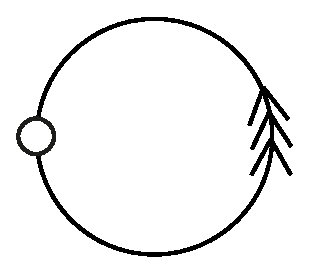
\includegraphics[scale=0.2]{4-01}\\ \hline 
	\multicolumn{3}{c}{ $\downarrow$ $\mathbb{Z}_2$ orbifold} \\ \hline
	$\mathbb{C}^3/\mathbb{Z}_2$ & $2$ & 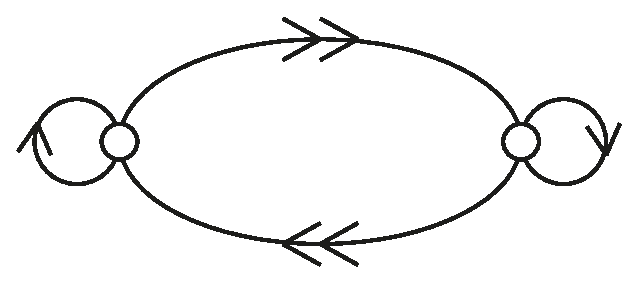
\includegraphics[scale=0.2]{2-01} \\ \hline
	\multicolumn{3}{c}{ $\downarrow$ mass reduction} \\ \hline
	Klebanov-Witten & $1$ & 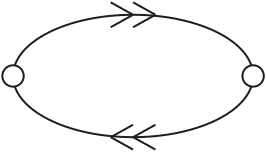
\includegraphics[scale=0.2]{1-01}\\ \hline
	\multicolumn{3}{c}{ $\downarrow$ $\mathbb{Z}_2$ orbifold} \\ \hline
	$Y^{2,0}$ & $1$ & 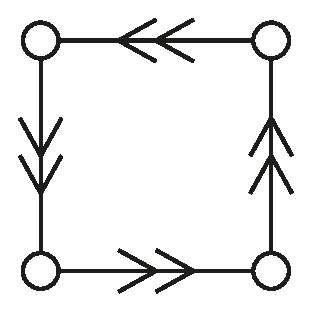
\includegraphics[scale=0.2]{3-01}\\ \hline
\end{tabular}
\end{center}

The transformations turning each theory into the next will be explained progressively.

\section{Brane stack in $\mathbb{C}^3$ and $\mathcal{N}=4$ super-Yang-Mills} \label{SYM4}

If $X_6 = \mathbb{C}^3$, the branes are invariant under half of the $16 \times 2 = 32$ IIB supercharges. This implies $\mathcal{N}=4$ for the field theory. Moreover, the theory features gluons as the massless spin-1 modes for the sector of strings stretching between brane $i$ and brane $j$ so that the gauge group is $U(N)$, as seen in \ref{sec:branestacks}. The information that the theory is a $U(N)$ gauge theory and is maximally supersymmetric is enough to uniquely fix it. Actually, since our main interest is in the IR limit, the $U(1)$ gauge factor decouples as we have explained in general, and the group is reduced to $SU(N)$.

In $\mathcal{N}=1$ language (which we employ even though the model has $\mathcal{N}=4$) the theory describes the dynamics of an $U(N)$ gauge vector supermultiplet $V_\mu$ and three complex chiral superfields $(X^a)_{i\dot j}$, $a=1,2,3$ in the adjoint of the gauge group (we will frequently omit gauge indices). These are nothing else than the parametrization of the D3-branes' position in $\mathbb{C}^3$ and therefore transform in the fundamental of $SU(3)$. The superpotential is the only one allowed by gauge and $SU(3)$ invariance,

\begin{equation} W(X) = g \epsilon_{abc} \Tr ( X^a X^b X^c) \label{sym4potential}\,;
\end{equation}

note the coupling $g$ is also the coupling of the gauge group, not an indipendent parameter. Since the theory has a single $SU(N)$ factor in the gauge group, and three fields in the adjoint (which is trivially a bifundamental with the same node at the two ends), the quiver diagram is rather simple:

\tikzset{% arrow close to the source: the 0.2 determines where the arrow is drawn
  ->-/.style={decoration={markings, mark=at position 0.5 with {\arrow{stealth}}},
              postaction={decorate}},
}

\begin{figure}[H]
	\centering
%\begin{tikzpicture}[every node/.style={circle,draw},thick,scale=1.5]
%  \node(NL) at (0,0){};
%  \draw[->-](NL.north) to [loop above, min distance=20mm, in=-45, out=45, looseness=8]	(NL.south);
%  \draw[->-](NL.north) to [loop above, min distance=24mm, in=-45, out=45, looseness=8]	(NL.south);
%  \draw[->-](NL.north) to [loop above, min distance=28mm, in=-45, out=45, looseness=8]	(NL.south);
%\end{tikzpicture}
	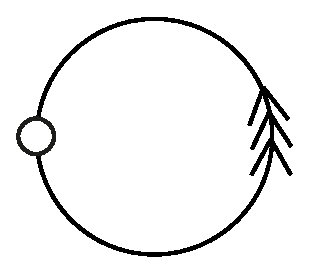
\includegraphics[scale=0.5]{4-01}
\end{figure}


Note that the obvious global symmetries, the $U(1)$ R-charge for $\ssn = 1$ and the $SU(3)$ flavour symmetry acting on the $X^a$ are actually just a subgroup of a $SU(4)$ R-symmetry group for the hidden $\ssn = 4$ supersymmetry. To make this manifest, split the $\ssn=1$ superfields as $V_\mu = (A_\mu,\lambda)$ and $X^a = (\phi^a,\psi^a)$, and regroup the fields as

\begin{align}
	\lambda^\alpha := (\lambda,\psi^1,\psi^2,\psi^3)\,,\quad \phi^i =: \varphi^i + i \varphi^{i+3}\,,
	\label{}
\end{align}

then $(A_\mu,\lambda^\alpha,\varphi^i)$ form an $\ssn=4$ vector supermultiplet, the components transforming respectively as $\mathbf{1}$, $\mathbf{4}$, $\mathbf{6}$ under $SU(4)$, and in the adjoint of gauge $SU(N)$.

$\ssn = 4$ (maximal) supersymmetry is extremely constraining, and indeed a non-renormalization theorem (first proven nonperturbatively in \cite{seibergnr}) states the theory is exactly finite. No divergences means the $\beta$ function (one for the only gauge coupling) vanishes identically, and the theory is always superconformal. Indeed, there is a set of additional 16 supercharges beyond the standard ones. These do \emph{not} however find a direct correspondence as supersymmetries of the D3-brane system, but only of the ``near-horizon'' ($\alpha' \rightarrow 0$) geometry of the brane stack.

The conformal manifold of such a theory is minimal: there is a single marginal deformation corresponding to changing $\tau$, as we know the theory is a SCFT for every value of the coupling, and there is no freedom associated with the superpotential as it is essentially fixed by the $X^a$ being combined into an $\ssn = 4$ multiplet with the gauge field.

The moduli space is also very easy to describe. The F-term conditions simply read:

\begin{equation}
	\pder{W}{X^a} \propto \varepsilon_{abc} X^b X^c = 0\,,
	\label{}
\end{equation}

so that the space of solution is given by (VEVs of) $X^a$ that commute with eachother as $N\times N$ matrices. Therefore, they can be simultaneously diagonalized by a gauge transformation, and the $3N$ eigenvalues $x^a_I$, $I=1,\ldots,N$ are completely free. In fact, these coincide directly with the coordinates of the $N$ D3-brane on $\mathbb{C}^3$. The moduli space is $\mathbb{C}^{3N}$, or to be precise, taking into account brane indistinguishability (i.e., the residual permutation gauge symmetry after diagonalization of the $X^a$),

\begin{equation}
	\mathcal{M} = \mathcal{M}_\text{mes} = \operatorname{Sym}^N \mathbb{C}^3\,.
	\label{}
\end{equation}

As predicted, there are no independent baryons and the moduli space coincides with the mesonic one. Accordingly, there are no deformations of the Calabi-Yau structure of $\mathbb{C}^3$.

\section{$\mathbb{C}^3/\mathbb{Z}_2$ orbifold}

We now move to a less trivial case by performing an orbifold of the background. Essentially, we act on $\mathbb{C}^3$ as such

\begin{equation}
	(z^1, z^2, z^3) \mapsto (-z^1, -z^2, z^3)
	\label{}
\end{equation}

and quotient under this $\mathbb{Z}_2$ group. This yields a Calabi-Yau manifold with a conical singularity in $z^1 = z^2 =0$. Equivalently, if the background is presented in polar coordinates as $\mathbb{R}_+ \times \mathbb{S}^5$, the orbifold produces $\mathbb{R}_+ \times (\mathbb{S}^5 / \mathbb{Z}_2)$. Our interested is then for the worldvolume theory of $N$ D3-branes placed in this singular background.

To investigate this, we consider $\tilde N = 2N$ D3-branes on $\mathbb{C}^3$, producing SYM4 as seen in the previous section, then we act on the $A_\mu$ and $X^a$ fields with the $\mathbb{Z}_2$ action and select the subset of invariant fields - these will be the degrees of freedom of the orbifold theory.

We need to specify an action of $\mathbb{Z}_2$ on the gauge indices. The following choice is convenient: act on an object in the fundamental $\mathbf{\tilde N} = \mathbf{N} \oplus \mathbf{N}$ as $1$ on the first factor and $-1$ on the second. This means, for example, that having decomposed $A_\mu$ in subrepresentations its transformation under $\mathbb{Z}_2$ is

\begin{equation}
	A_\mu = \begin{pmatrix}
		A^{0,0} & A^{1,0} \\
		A^{0,1} & A^{1,1}
	\end{pmatrix} \mapsto \begin{pmatrix}
		A^{0,0} & -A^{1,0} \\
		-A^{0,1} & A^{1,1}
	\end{pmatrix}\,,
\end{equation}

where $A^{i,j}$ are $N\times N$ matrices. We see the surviving gauge fields are $A^{0,0}$ and $A^{1,1}$, adjoint for the $U(N) \times U(N)$ subgroup of $U(2\tilde N)$. The new gauge group is therefore $U(N) \times U(N)$.

The same holds for $X^3$, which becomes $\Phi := (X^3)^{0,0}$ and $\tilde \Phi := (X^3)^{1,1}$, two chiral fields each in the adjoint of one of the $U(N)$ factors.

For $X^1$, $X^2$ instead one has to take into account both the action on the gauge indices and the direct action on the $\mathbb{C}^3$ geometry. With $i=1,2$, one has

\begin{equation}
	X^i = \begin{pmatrix} 
			(X^i)^{0,0} & (X^i)^{1,0} \\
			(X^i)^{1,0} & (X^i)^{1,1} 
		\end{pmatrix}\mapsto \begin{pmatrix} 
			-(X^i)^{0,0} & (X^i)^{1,0} \\
			(X^i)^{1,0} & -(X^i)^{1,1} 
		\end{pmatrix}\,,
\end{equation}

and one ends up with two pairs of chiral fields in bifundamentals, $A^i := (X^i)^{0,1}$, $B^i := (X^i)^{1,0}$, in representations $(\rrep N, \cjrep N)$ and $(\cjrep N, \rrep N)$ of $U(N)\times U(N)$ respectively. The structure of the theory can be more elegantly presented in a quiver diagram:

\begin{figure}[H]
	\centering
%\begin{tikzpicture}[every node/.style={circle,draw},thick,scale=1.5]
%  \node(NL) at (0,0){};
%  \node(NR) at (2,0){};
%  \draw[->-](NL.north) to [bend left=60]	(NR.north);
%  \draw[->-](NL.north) to [bend left=90]	(NR.north);
%  \draw[->-](NR.south) to [bend left=60]	(NL.south);
%  \draw[->-](NR.south) to [bend left=90]	(NL.south);
%  \draw[->-] (NL.south west) to [loop left, min distance=5mm, in=120, out=230, looseness=10] (NL.north west);
%  \draw[->-] (NR.south east) to [loop left, min distance=5mm, in=60, out=300, looseness=10] (NR.north east);
%\end{tikzpicture}
	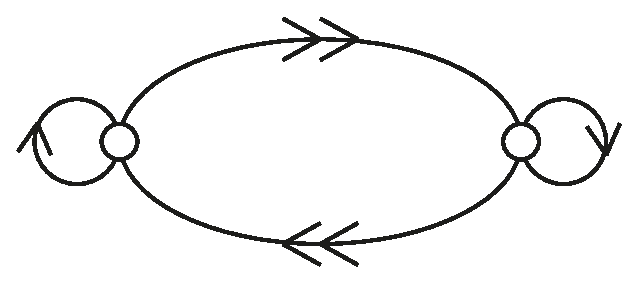
\includegraphics[scale=0.5]{2-01}
\end{figure}

The superpotential is just given by restriction of the SYM4 potential \eqref{sym4potential} to the surviving fields; after some algebra

\begin{equation}
	W = \mu \left( \Tr \Phi (A_1 B_1 + A_2 B_2 ) + \Tr \tilde\Phi (B_1 A_1 + B_2 A_2) \right)
	\label{}
\end{equation}

It is clear at this point that, given the introduction of an asymmetry between $X^3$ and $X^{1,2}$, the $\ssn = 4$ R-symmetry $SU(4)$ is broken and so is maximal supersymmetry. The orbifold theory has indeed $\mathcal{N}=2$ supersymmetry\cite{Douglas}.

%\cmmnt{--Tutto ci\`o che c'\`e qua sotto dove si trova?--}
%
%This theory, moreover, is also superconformal at some points. The form of the potential is again fixed (there are no possible deformation consistent with the remaining symmetries) except for the overall constant $\mu$; therefore a set of parameters for the theory is given by the three couplings $(\tau_1,\tau_2,\mu)$, where we have accounted for the fact that the two gauge factors can flow independently under the renormalization group. Then, the vanishing of the $\beta_\mu$ function for the $\mu$ coupling is equivalent the R-charge of the superpotential being $2$, so that
%
%\begin{equation}
%	R_\Phi + R_A + R_B = 2\,,\quad R_{\tilde\Phi} + R_A + R_B = 2
%	\label{}
%\end{equation}
%
%which, employing $\frac{3}{2}R = 1+\gamma$ for chiral fields at a superconformal point, is equivalent to
%
%\begin{equation}
%	\gamma_\Phi + \gamma_A + \gamma_B = 0 = \gamma_{\tilde \Phi} + \gamma_A + \gamma_B\,.
%	\label{}
%\end{equation}
%
%We combine this with the vanishing of the two gauge $\beta$ functions. Using the NSVZ formula for the left node we get
%
%\begin{equation}
%	\beta \propto 3N-N(1-2\gamma_\Phi) - 2 \frac{N}{2} ( 1-2\gamma_A) - 2 \frac{N}{2} (1- 2\gamma_B) = 2 ( \gamma_\Phi + \gamma_A + \gamma_B) = 0\,,
%	\label{}
%\end{equation}
%
%and identically for the other gauge node, replacing $\Phi$ with $\tilde\Phi$. Therefore the conformal conditions are not all independent: only two independent conditions determine the conformal manifold. Since we have a three parameter space $(\tau_1, \tau_2, \mu)$, the locus of conformal points will be 1-dimensional. At a generic point $(\tau_1,\tau_2,\mu)$ in parameter space the theory will not be superconformal; however it should flow in the IR towards a point on the conformal curve.
%
%Directions along the conformal manifolds are marginal deformations of the theory, as seen before. In this case, one marginal deformation will be present.
%
%\cmmnt{Moduli space? Forse $b_3(Y) = 0$?}

We will not concentrate on the details of this $\mathbb{C}^3/\mathbb{Z}_2$ theory; we use it as a stepping stone from SYM4 to the Klebanov-Witten theory, which we will introduce in the next section as a deformation of the orbifold theory.

\section{The conifold and the Klebanov-Witten model} \label{sec:KW}

In \cite{KW_SCFT} the case of $X_6$ being the conifold was studied. The conifold is a specific Calabi-Yau 3-cone defined for example as the following variety in $\mathbb{C}^4$:

\begin{equation}
	z_1^2 + z_2^2 + z_3^2 + z_4^2 = 0\,,
\end{equation}

with the K\"ahler structure inherited from the standard one on $\mathbb{C}^4$, or, after a simple change of variables:

\begin{equation}
	u v - xy = 0\,.
	\label{}
\end{equation}

The base can be found by quotienting by dilations $z_i \rightarrow \lambda z_i$ (with $\lambda \in \mathbb{R}_+$) and turns out to be the homogeneous space $SO(4)/U(1) = SU(2)\times SU(2) / U(1)$, where the $U(1)$ is a diagonal subgroup generated by, say, $T^3_L + T^3_R$. Topologically, this is $\mathbb{S}^2 \times \mathbb{S}^3$. We will therefore have $SU(2)\times SU(2)$ as part of the isometry group of both $Y_5$ and $X_6$, and thus will also appear as a global symmetry of the wordvolume theory. An equivalent description of the topology of the conifold is as a $U(1)$ bundle over $\mathbb{C}P^1 \times \mathbb{C}P^1 \cong \mathbb{S}^2 \times \mathbb{S}^2$; in these terms the metric on the base that makes the cone Calabi-Yau is

\begin{equation}
	ds^2_5 = \frac{1}{9} (d\psi + \cos\theta_1 d\phi_1 + \cos\theta_2 d\phi_2)^2 + \frac{1}{6} (d\Omega_1^2 + d\Omega_2^2)
\end{equation}

where $\Omega_i^2 = d\theta_i^2 + \sin\theta_i^2 d\phi_i^2$ is the metric on the $\mathbb{C}P^1_i$, and $\psi$ is the fibral coordinate with period $4\pi$.

The corresponding field theory (which we will call the Klebanov-Witten model), however, can also be found by applying a particular modification to the orbifold theory of the previous section\cite{KW_SCFT}. Let us derive the form of this SCFT in this way, and then show how the above geometry reappears from the field theory side. The modification is the addition of a relevant term to the Lagrangian, a mass for the $\Phi$, $\tilde\Phi$ adjoint fields

\begin{equation}
	\mathcal{M} = \frac{M}{2} \left( \Tr \Phi^2 - \Tr \tilde\Phi^2 \right)\,,
	\label{massterm}
\end{equation}

thus providing a possible UV completion for the $\mathbb{C}^3/\mathbb{Z}_2$ theory. These fields are then eliminated using the resulting classical equations of motion. For example,

\begin{equation}
	\pder{(\mathcal{M} + W)}{\Phi} = 0 \Rightarrow \Phi = - \frac{\mu}{M} \left( A_1 B_1 + A_2 B_2 \right)
	\label{}
\end{equation}

and analogously for $\tilde \Phi$. Finally, these are substituted back into the action, reducing the chiral fields to just $A_i$ and $B_i$ and the superpotential to

\begin{equation}
	W = \frac{\lambda}{2} \epsilon^{ij} \epsilon^{kl} \Tr \left( A_i B_k A_j B_l \right)
	\label{kwpotential}
\end{equation}

having defined $\lambda := \frac{\mu^2}{2M}$. More formally, it is argued that after the introduction of the relevant term \eqref{massterm} the $\mathbb{C}^3/\mathbb{Z}_2$ theory flows in the IR to the Klebanov-Witten model.

Therefore, the worldvolume gauge theory is a $U(N)\times U(N)$ field theory featuring two chiral doublets $A_i$, $B_j$ with $i,j = 1,2$ transforming in opposite bifundamentals, that is $A_i$ in $(N,\bar N)$ and $B_j$ in $(\bar N, N)$. The quiver diagram is simpler:

\begin{figure}[H]
	\centering
%\begin{tikzpicture}[every node/.style={circle,draw},thick,scale=1.5]
%  \node(NL) at (0,0){};
%  \node(NR) at (2,0){};
%  \draw[->-](NL.north) to [bend left=60]	(NR.north);
%  \draw[->-](NL.north) to [bend left=90]	(NR.north);
%  \draw[->-](NR.south) to [bend left=60]	(NL.south);
%  \draw[->-](NR.south) to [bend left=90]	(NL.south);
%\end{tikzpicture}
	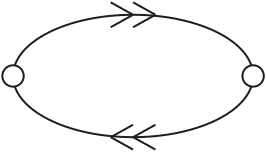
\includegraphics[scale=0.5]{1-01}
\end{figure}

The $i$ and $j$ indices, instead, are acted upon respectively by the global left and right $SU(2)$ symmetries. From the form of the superpotential and these symmetries, furthermore, it is possible to deduce the R-charges of $A_i$ and $B_i$ are $1/2$, implying a dimension of $\Delta = 3/4$ when the theory is conformal. A non-canonical scaling dimension is a symptom that the CFT will always be strongly-coupled.

It is also clear the supersymmetry has been broken further to $\ssn = 1$, since \eqref{massterm} is not $\ssn = 2$ invariant ($\Phi$, $\tilde \Phi$ were actually combined with $A_i$, $B_i$ into $\ssn = 2$ hypermultiplets in the orbifold theory). The case at hand is thus a four-dimensional strongly-coupled field theory with minimal supersymmetry.

The Klebanov-Witten theory will also not be in general superconformal; it will flow through renormalization in the IR to a conformal submanifold in the space of couplings $(\lambda,\tau_1,\tau_2)$, the locus where the $\beta$ functions for these three couplings vanish. It turns out these three conditions are all equivalent. In particular, requiring $\beta_{\tau_1} = 0$ and making use of \eqref{nszv} this unique condition is equivalent to

\begin{equation}
	3 T[\mathrm{Adj}] - \sum_i T[R_i] ( 1- 2\gamma_i) = 0
	\label{}
\end{equation}

When evaluating this, care should be taken with the fact that $A_i$ and $B_j$ have a $U(N)_2$ index which is uncharged under $U(N)_1$ and must be summed over. Noting $\gamma_{A_1} = \gamma_{A_2}$ and $\gamma_{B_1} = \gamma_{B_2}$ because of the global symmetry, this gives (for both nodes)

\begin{equation}
	\gamma_A + \gamma_B + \frac{1}{2} = 0\,.
	\label{}
\end{equation}

Being $\gamma_{A,B}$ functions of the couplings, this equation defines a critical 2-surface in parameter space. Switching to R-charges, this means

\begin{equation}
	R_A + R_B = 1\,,
	\label{}
\end{equation}

but this is also the vanishing of the $\beta$ function for the superpotential coupling $\lambda$, since $R_W = 2$ is just

\begin{equation}
	R_A + R_B + R_A + R_B = 2\,.
	\label{}
\end{equation}

Thus, since the three conditions are equivalent, the final conformal manifold is the locus of a single equation in three variables $(\lambda,\tau_1,\tau_2)$ and is thus two-dimensional. Therefore there will be two marginal deformations of the theory.

Let us comment briefly on the whereabouts of the abelian gauge factors of $U(N) \times U(N)$ under RG flow towards the infrared. Denoting as $T^1$ and $T^2$ the generators of the two trace $U(1)$ of the left and right nodes, it is clear $T^1+T^2$ is the overall completely decoupled $U(1)$ that we can safely ignore. The only remaining abelian factor is generated by $B = T^1 - T^2$. This symmetry is non-anomalous and thus flows into a rigid $U(1)$ in the IR. We call this charge, corresponding to the symmetry

\begin{equation}
	A_i \rightarrow e^{i\theta} A_i\,,\quad B_i \rightarrow e^{-i\theta} B_i
	\label{}
\end{equation}

a baryon number.

Position in moduli space $\mathcal{M}$ should be parametrized by the expectation values of gauge-invariant operator (hadrons). In particular, the classical moduli space is given by the F-term and D-term conditions, which specialized to the particular case are

\begin{equation}
	\epsilon^{ij} A_i B_a A_j = \epsilon^{ij} B_i A_a B_j = 0
	\label{}
\end{equation}

\begin{equation}
	A_i A_i^\dagger - B_i B_i^\dagger = A^\dagger_i A_i - B^\dagger_i B_i = \xi \mathbbm{1}
	\label{}
\end{equation}

the equation have to be understood to hold for VEVs. Note the first and second D-term condition are respectively from the left and right gauge group. We set temporarily $\xi = 0$ to study the mesonic moduli space $\mathcal{M}_\text{mes}$. To reinterpret the F-flatness condition, we introduce the four matrices $\Phi_{ij} = A_i B_j$ and note

\begin{align}
	\left[ \Phi_{ij} , \Phi_{jk} \right] = 0\\
	\Phi_{11} \Phi_{22} = \Phi_{21}\Phi_{12}
	\label{}
\end{align}

which can be immediately checked to follow from the vanishing of the F-term. Since these commute, they can be simultaneously diagonalized and their $N$ eigenvalues (one for each brane) satisfy the conifold's equation:

\begin{equation}
	\phi^I_{11} \phi^I_{22} = \phi_{21}^I \phi_{12}^I
	\label{}
\end{equation}

so these quite literally parametrize the motion of the $N$ D3-branes on the background cone. These actually determine the VEVs of mesonic operators, mesons\footnote{The meson/baryon terminology is meant to be a direct generalization of the concept of QCD hadrons. A QCD meson is to a first approximation built from two quarks as a symmetric product $\ket{M} \sim \delta^i_{\,j} \ket{q^i \overline q_j} + \mathcal O (gluons)$, while a baryon is $\ket{B} \sim \epsilon_{ijk} \ket{q^i q^j q^k}$. In general, $SU(N)$-singlets can be built by contracting gauge indices either with the symmetrical $\delta^i_j$ or the antisymmetric $\epsilon_{a_1 \ldots a_N}$.} being generated by prototipical trace operators:

\begin{equation}
	M_{(ab\ldots),(ij\ldots)} =	\Tr\left( (A_a B_i)(A_b B_j)\cdots \right)\,.
	\label{}
\end{equation}

Note mesons are built by tracing over closed loops in the quiver diagram to make a gauge-invariant operator. All of these operators are actually expressable as products of $\Phi$ matrices, and as it was shown, only $3$ out of $4$ of those are independent. In the end, there are (accounting for gauge indices) $3N$ independent mesons whose VEVs parametrize mesonic moduli space, coincident with the $\operatorname{Sym}^N C$, where $C$ is the conifold.\\

Operators of non-zero baryon number can also be constructed by using the antisymmetric invariant gauge tensor $\epsilon^{a_1\ldots a_N}$, as such:

\begin{equation}
	B^A_{[k]} = \epsilon^{a_1\ldots a_N} \epsilon_{b_1\ldots b_n} (A_1)_{a_1}^{b_1} \ldots (A_1)^{a_k}_{b_k} (A_2)^{a_{k+1}}_{b_{k+1}} \ldots (A_2)^{b_N}_{a_N}
	\label{}
\end{equation}

where we have displayed gauge indices on the $A$ fields. There are only $N+1$ different assignment for the $SU(2)$ indices because of antisymmetry, so that there are $N+1$ fundamental baryons of the form of $B^A$. The same could be done by swapping the two gauge groups and using $B$ fields, to get additional $N+1$ $B^B$ baryons. These all have baryon number $N$ under the $U(1)$ baryonic symmetry

\begin{equation}
	A_i \rightarrow e^{i\theta} A_i\,,\quad B_j \rightarrow B e^{-i\theta}B_j\,,
	\label{}
\end{equation}

while mesons have baryon number $0$. This $U(1)$ symmetry can be proven to be non-anomalous\cmmnt{ref da MZ}.

All gauge-invariant operators in the theory are built out of these fundamental mesons, fundamental baryons, and their respective antiparticles (made out of the conjugate fields $A^\dagger$, $B^\dagger$. However, as we have anticipated, we only expect $g-1 = 1$ baryonic VEV to be independent. This VEV will be associated with the resolution of the cone singularity into a $\mathbb{CP}^1 \cong \mathbb{S}^2$, and will essentially coincide with $\xi$. To see an example of this deformation of the background geometry, let us set $\xi$ to a constant nonzero value. Then hypothesizing the $A_1, A_2, B_1, B_2$ matrices commute, applying F-term conditions we get that each set of eigenvalues satisfies

\begin{equation}
	a_1/a_2 = b_1/b_2
	\label{}
\end{equation}

So that $a_i$ and $b_i$ are proportional vectors of $\mathbb{C}^2$, therefore

\begin{equation}
	a_i = a e^{i\theta_A} n_i, \quad \quad b e^{i\theta_B} n_i
	\label{}
\end{equation}

where $a,b$ are real and $n_i$ belongs to a $\mathbb{CP}^1$. The phases are cancelled by modding gauge invariance, and $a$ and $b$ then are involved in the D-term:

\begin{equation}
	a^2 - b^2 = \xi
	\label{}
\end{equation}

so that essentially our mesonic VEVs are composed of $N$ copies of one non-compact radial coordinate (say, $a$) and a point on $\mathbb{CP}^1$. This means the conical singularity has disappeared to be replaced by a two-cycle on which the branes can move.\\

The explicit form of the baryon generating this deformation in terms of the fundamental hadrons is very challenging to determine\cite{Forcella}; fortunately, we will not need it for our purposes. In any case, all of this information will be clarified in the context of holography.

\section{The $Y^{(2,0)}$ orbifold theory}\label{sec:squares}

The same construction on a $\mathbb{Z}_2$ orbifold of the conifold yields a quiver gauge theory which will be the main interest of this work. The geometry of the base of the cone is very simply introduced in polar coordinates as 

\begin{equation}
	ds^2_5 = \frac{1}{9} (d\psi + \cos\theta_1 d\phi_1 + \cos\theta_2 d\phi_2)^2 + \frac{1}{6} (d\Omega_1^2 + d\Omega_2^2)
\end{equation}

i.e., exactly the same metric in form as the conifold, but with $\psi$ now with period $2\pi$. This background and the resulting worldvolume field theory are just one entry $Y^{2,0}$ of an infinite class $Y^{p,q}$ of examples introduced in \cite{benvenutiInfinite}.

Following an identical procedure to that performed for the $\mathbb{Z}_2$ orbifold of SYM4, we can deduce the quiver diagram splits to yield four doublets of bifundamental chiral fields stretching in a square between four nodes:

\begin{figure}[H]
	\centering
%\begin{tikzpicture}[every node/.style={circle,draw},thick,scale=1.5]
%  \node(NL) at (0,0){};
%  \node(NR) at (2,0){};
%  \node(NDR) at (2,2){};
%  \node(NDL) at (0,2){};
%  \draw[->-](NL.east) to [bend right=20]	(NR.west);
%  \draw[->-](NL.east) to [bend left=20]	(NR.west);
%  \draw[->-](NR.north) to [bend right=20]	(NDR.south);
%  \draw[->-](NR.north) to [bend left=20]	(NDR.south);
%  \draw[->-](NDR.west) to [bend right=20]	(NDL.east);
%  \draw[->-](NDR.west) to [bend left=20]	(NDL.east);
%  \draw[->-](NDL.south) to [bend right=20]	(NL.north);
%  \draw[->-](NDL.south) to [bend left=20]	(NL.north);
%\end{tikzpicture}
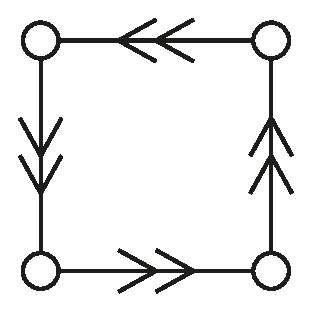
\includegraphics[scale=0.5]{3-01}
\end{figure}

and the superpotential can be again obtained by truncation, yielding

\begin{equation}
	W = \lambda \epsilon^{ij} \epsilon^{kl} \Tr\left( A_i B_k C_j D_l \right)
	\label{}
\end{equation}

from which it is clear that the $SU(2) \times SU(2)$ isometry of the cone, corresponding to a global symmetry of the field theory, must now act with the left factor on $A_i$ and $C_i$, and the right on $B_i$ and $D_i$. 

The novelty in this model is the appearance of an anomalous $U(1)$. In detail, of the four gauge $U(1)$s, one (the symmetric sum) is the overall trace and decouples completely. It turns out that the three remaining abelian factors are partitioned into one non-anomalous baryonic $U(1)$ (which is inherited directly from the KW model) and two new anomalous $U(1)$s.

We turn to the study of marginal deformations. This time three of the four gauge $\beta$ functions are independent:

\begin{equation}
	\begin{split}
	\gamma_A + \gamma_D + \frac{1}{2} = 0 \\
	\gamma_B + \gamma_A + \frac{1}{2} = 0 \\
	\gamma_C + \gamma_B + \frac{1}{2} = 0 
	\end{split}
\end{equation}

$\beta_\lambda = 0$ is also not independent. At any superconformal point, $\frac{3}{2}R - 1 = \gamma$, so that the condition that $W$ be scale invariant, which is equivalent to it having R-charge $2$, becomes

\begin{equation}
	\begin{split}
	2 = R_W = R_A + R_B + R_C + R_D \\\Rightarrow \gamma_A + \gamma_B + \gamma_C + \gamma_D + 1 = 0
	\label{}
\end{split}
\end{equation}

which is indeed equivalent to the above system. Three independent equations in the five-parameter space of $(\tau_1,\tau_2,\tau_3,\tau_4,\lambda)$ define, again, a critical 2-submanifold.

Turning to the investigation of the moduli space, the F-term condition for the given superpotential read

\begin{align}
	\begin{split}
	A_\alpha B_\sigma C_\beta \epsilon^{\alpha\beta} = 0 \\
	B_\alpha C_\sigma D_\beta \epsilon^{\alpha\beta} = 0 \\
	C_\alpha D_\sigma A_\beta \epsilon^{\alpha\beta} = 0 \\
	D_\alpha A_\sigma B_\beta \epsilon^{\alpha\beta} = 0 
	\label{}
\end{split}
\end{align}

while the vanishing of the D-term takes the form

\begin{align}
	\begin{split}
		A_i A^\dagger_i - B_i B^\dagger_i = \xi_1 \mathbbm{1} \\
		B_i B^\dagger_i - C_i C^\dagger_i = \xi_2 \mathbbm{1} \\
		C_i C^\dagger_i - D_i D^\dagger_i = \xi_3 \mathbbm{1} \\
		D_i D^\dagger_i - A_i A^\dagger_i = \xi_4 \mathbbm{1}
	\end{split}
	\label{}
\end{align}

with the constraint $\sum_i \xi_i = 0$ (obvious by summing the four equations). To sketch out mesonic moduli space, again we make the simplifying assumption the eight $A, B, C, D$ matrices commute and can be simultaneously diagonalized. So, for each of the $N$ rows of corresponding eigenvalues,

\begin{align}
	a_1/a_2 = c_1/c_2 && b_1/b_2 = d_1 / d_2
	\label{}
\end{align}

thus again $a_\alpha \propto c_\alpha$ and $b_\alpha \propto d_\alpha$, so we can ``projectivize'':

\begin{align}
		a_\alpha = a \, e^{i\theta_A} n_\alpha && b_\alpha = b \, e^{i\theta_B} n_\alpha \\
		c_\alpha = c \, e^{i\theta_C} m_\alpha && d_\alpha = d \, e^{i\theta_D} m_\alpha 
\end{align}

and again the phases are modded out by gauge symmetry, and the $a, b, c, d$ real numbers are reduced to a single coordinate (schematically $r^2$) by the three independent D-flatness conditions. Therefore the resolved geometry of the singularity is now $\mathbb{CP}^1 \times \mathbb{CP}^1$, with a clear correspondence with the explicit metric of the resolved $Y^{2,0}$, which is the general Calabi-Yau deformation of the latter. This is found to be\cite{copycit}

\begin{equation}
	\begin{split}
	ds^2 = \kappa^{-1}(r) dr^2 + \frac{1}{9} \kappa(r) r^2 \left( d\psi + \cos\theta_1 d\varphi_1 + \cos\theta_2 d\varphi_2 \right)^2 \\
	+ \frac{1}{6} r^2 d\Omega_1^2 + \frac{1}{6}(r^2 + a^2) d\Omega_2^2\,,
	\label{genCYy20cones}
\end{split}
\end{equation}

\begin{equation}
	\kappa(r) = \frac{1 + \frac{9a^2}{r^2} - \frac{b^6}{r^6}}{1 + \frac{6a^2}{r^2}}\,.
	\label{}
\end{equation}

It can be seen that the singular $Y^{2,0}$ cone is obtained as the two moduli $a$, $b$ vanish. If, instead, they do not, the conical singularity is ``resolved'', similar to the case of the conifold, and the resolved tip of the cone\footnote{This does not actually lie at $r=0$ because of the way the $r$ coordinate is defined, rather it corresponds to $\kappa(r) = 0$; we will clarify this in our study of the $Y^{2,0}$ resolved geometry in chapter \ref{chap:y20}} is $\mathbb{S}^2 \times \mathbb{S}^2$, with (combinations of) $a$ and $b$ parametrizing the volumes of the two spheres.

In this case, the presence of $g-1 = 3$ independent $\xi$ parameters (matching with three independent baryons) should perplex, as the resolution of the singularity should be controlled by the \emph{two} volumes of the spheres. In fact, the general Calabi-Yau deformation of the $Y^{2,0}$ metric will indeed depend on two moduli. In this case, the third modulus is not interpretable as due to deformation of the background metric, but is actually connected to the moduli of IIB two-form fields. We will review this fact in a holographic context.

For completeness we adapt the construction of hadronic operators. We note fundamental mesons are now built using $ABCD$ loops (omitting $SU(2)^2$ indices):

\begin{equation}
	M = \Tr \left( (ABCD)(ABCD) \ldots \right)
	\label{}
\end{equation}

and four classes of fundamental baryons can be introduced as before

\begin{equation}
	B^A = \epsilon^{a_1\ldots a_n}\epsilon_{b_1 \ldots b_n} A^{b_1}_{a_1} \ldots A^{b_n}_{a_n}
	\label{}
\end{equation}

and this can be repeated for $B$, $C$, $D$. Similarly to the previous case, we expect only three baryons to be truly indepedent and a suitable triple of combinations should generate the three aforementioned flat shifts.



